\documentclass[a4paper, 14pt]{extarticle}
\usepackage[russian]{babel}
\usepackage[T1]{fontenc}
\usepackage{fontspec}
\usepackage{indentfirst}
\usepackage{enumitem}
\usepackage{graphicx}
\usepackage[
  left=20mm,
  right=10mm,
  top=20mm,
  bottom=20mm
]{geometry}
\usepackage{parskip}
\usepackage{titlesec}
\usepackage{xurl}
\usepackage{hyperref}
\usepackage{float}
\usepackage[
  figurename=Рисунок,
  labelsep=endash,
]{caption}
\usepackage[outputdir=build, newfloat]{minted}

\hypersetup{
  colorlinks=true,
  linkcolor=black,
  filecolor=blue,
  urlcolor=blue,
}

\renewcommand*{\labelitemi}{---}
\setmainfont{Times New Roman}
\setmonofont{JetBrains Mono}[
  SizeFeatures={Size=11},
]

\newenvironment{code}{\captionsetup{type=listing}}{}
\SetupFloatingEnvironment{listing}{name=Листинг}

\setminted{
  fontsize=\footnotesize,
  frame=lines,
  framesep=2mm,
}

\setminted[text]{
  frame=none,
}

\setlength{\parskip}{6pt}

\setlength{\parindent}{1cm}
\setlist[itemize]{itemsep=0em,topsep=0em,parsep=0em,partopsep=0em,leftmargin=2.0cm,wide}
\setlist[enumerate]{itemsep=0em,topsep=0em,parsep=0em,partopsep=0em,leftmargin=2.0cm,wide}

\renewcommand{\thesection}{\arabic{section}.}
\renewcommand{\thesubsection}{\thesection\arabic{subsection}.}
\renewcommand{\thesubsubsection}{\thesubsection\arabic{subsubsection}.}

\titleformat{\section}{\normalfont\bfseries}{\thesection}{0.5em}{}
\titleformat{\subsection}{\normalfont\bfseries}{\thesubsection}{0.5em}{}

\titleformat*{\section}{\normalfont\bfseries}
\titleformat*{\subsection}{\normalfont\bfseries}

\linespread{1.5}
\renewcommand{\baselinestretch}{1.5}

\begin{document}

\begin{titlepage}
  \vspace{0pt plus2fill}
  \noindent

  \vspace{0pt plus6fill}
  \begin{center}
    Санкт-Петербургский национальный исследовательский университет
    информационных технологий, механики и оптики

    \vspace{0pt plus3fill}

    Факультет инфокоммуникационных технологий

    Направление подготовки 11.03.02

    \vspace{0pt plus2fill}

    Лабораторная работа №2

    Использование Git и Gulp \\ для решения задач web-разработки

  \end{center}

  \vspace{0pt plus9fill}
  \begin{flushright}
    Выполнил: \\
    Швалов Даниил Андреевич

    Группа: К33211

    Проверила: \\
    Марченко Елена Вадимовна
  \end{flushright}

  \vspace{0pt plus2fill}
  \begin{center}
    Санкт-Петербург

    2023
  \end{center}
\end{titlepage}

\section{Введение}

\textbf{Цель работы}: научиться использовать систему контроля версий Git для
отслеживания и ведения истории изменения файлов в проектах, познакомиться с
инструментом для автоматизации, организации и обработке задач Gulp, разработать
собственное приложение для просмотра веб-страниц.

\section{Ход работы}

\subsection*{Задание №1}

В данном задании необходимо установить Git на компьютер, настроить на работу с
проектом, выполнить изменения в файлах проекта. Для выполняемых изменений
сделать коммиты (не менее трех). Проверить, что коммиты создаются. Локальный
репозиторий синхронизировать с удаленным.

В качестве файлов, которые будут отслеживаться системой контроля версий Git,
были выбраны файлы проектов всех лабораторных работ по веб-программированию. С
помощью команды \texttt{git init}, выполненной в корне проекта, был
инициализирован репозиторий. С помощью команды \texttt{git add} все интересующие
файлы были помечены как отслеживаемые. После этого была использована команда
\texttt{git commit -m "message"} для фиксации изменений. Вместо \texttt{message}
были использованы сообщения, описывающие изменения в данной фиксации.

После проделанных действий было необходимо синхронизировать локальный
репозиторий с удаленным. В качестве удаленного репозитория был выбран GitHub,
поскольку это популярная площадка для хранения кода, обладающая богатым
функционалом для разработчиков. Для GitHub существует множество руководств, что
позволяет быстро найти ответ на нужный вопрос. В добавок ко всему, GitHub
позволяет бесплатно создавать сколь угодно большое количество публичных
репозиториев.

Для того, чтобы загрузить локальный репозиторий на GitHub,
\href{https://github.com/danilshvalov/itmo-web-programming}{был создан}
удаленный репозиторий на GitHub. После этого была выполнена следующая команда:
\begin{minted}{text}
  git remote add origin \
    https://github.com/danilshvalov/itmo-web-programming.git
\end{minted}
Данная команда устанавливает ссылку на удаленный репозиторий, с которым будет
синхронизирован локальный репозиторий. Чтобы отправить изменения на удаленный
репозиторий была выполнена команда \texttt{git push origin main}, которая
синхронизирует текущие изменения в ветке \texttt{main}.

В итоге все файлы, которые были помечены как отслеживаемые, были
синхронизированы с удаленным репозиторием (рис. \ref{fig:github-files}). На рис.
\ref{fig:github-commits} показана история фиксаций, отображаемая в интерфейсе
GitHub.

\begin{figure}[H]
  \centering
  \fbox{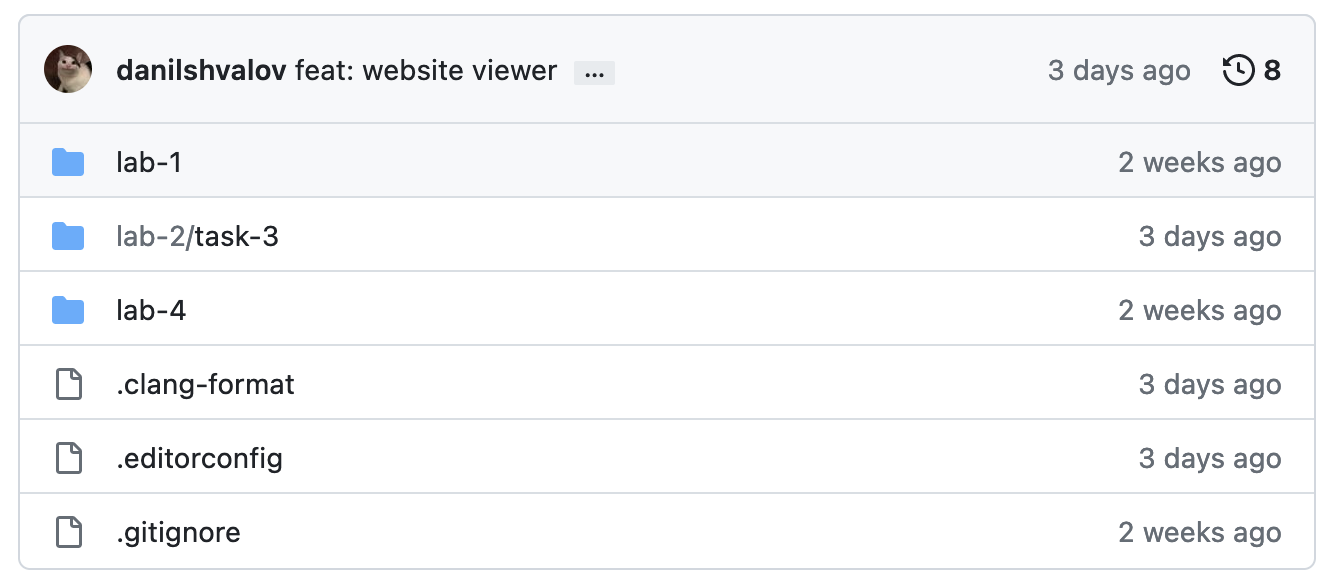
\includegraphics[width=\textwidth]{images/github-files.png}}
  \caption{Файлы на удаленном репозитории GitHub}
  \label{fig:github-files}
\end{figure}

\begin{figure}[H]
  \centering
  \fbox{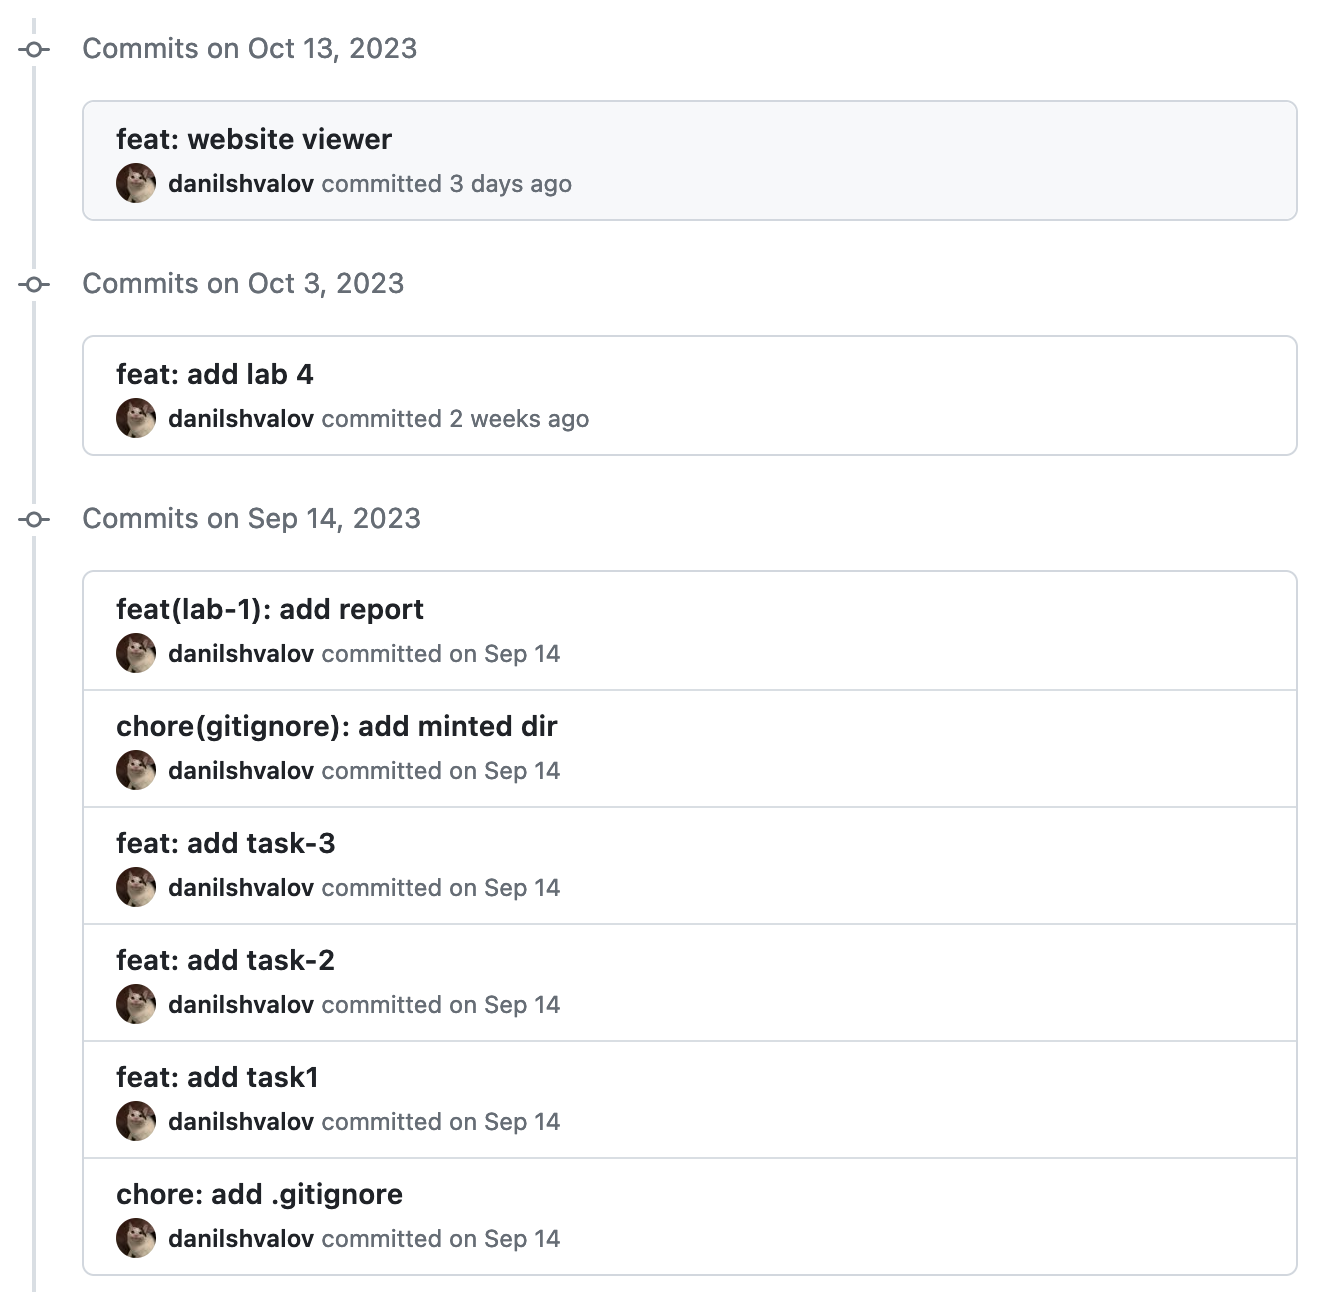
\includegraphics[width=\textwidth]{images/github-commits.png}}
  \caption{История фиксаций в интерфейсе GitHub}
  \label{fig:github-commits}
\end{figure}

\subsection*{Задание №2}

В данном задании необходимо установить Gulp, отметив этапы установки, а также
создать какой-нибудь task.

Для выполнения задания был инициализирован проект с помощью команды \texttt{npm
  init}. После выполнения команды в корне проекта появился файл
\texttt{package.json}, который содержит в себе информацию о проекте. Содержимое
этого файла находится в приложении \ref{app:package.json}.

После этого в проект был установлен Gulp с помощью команды \texttt{npm i gulp}.
Также с помощью команды \texttt{npm i browser-sync} был установлен BrowserSync —
утилита, которая автоматически перезагружает измененные файлы и страницы,
синхронизирует навигацию между браузерами, а также позволяет тестировать сайт
сразу на нескольких устройствах.

После установки в корне проекта был создан файл \texttt{gulpfile.js}, исходный
код которого находится в приложении \ref{app:gulpfile.js}. Данный файл создает
task с названием \texttt{browserSync}, который отслеживает изменения файлов и
обновляет браузер в случае, если файлы были изменены. Кроме того, был создан
task с названием \texttt{default}, чтобы было можно запускать Gulp не указывая в
аргументах название task. Также для тестирования Gulp был создан файл
\texttt{index.html}, исходный код которого находится в приложении
\ref{app:index.html}.

Для запуска Gulp необходимо выполнить команду \texttt{gulp} в эмуляторе
терминала. При выполнении этой команды запустится сервер, который будет
отслеживать изменения файлов (рис. \ref{fig:browser-sync} и
\ref{fig:browser-before}).

\begin{figure}[H]
  \centering
  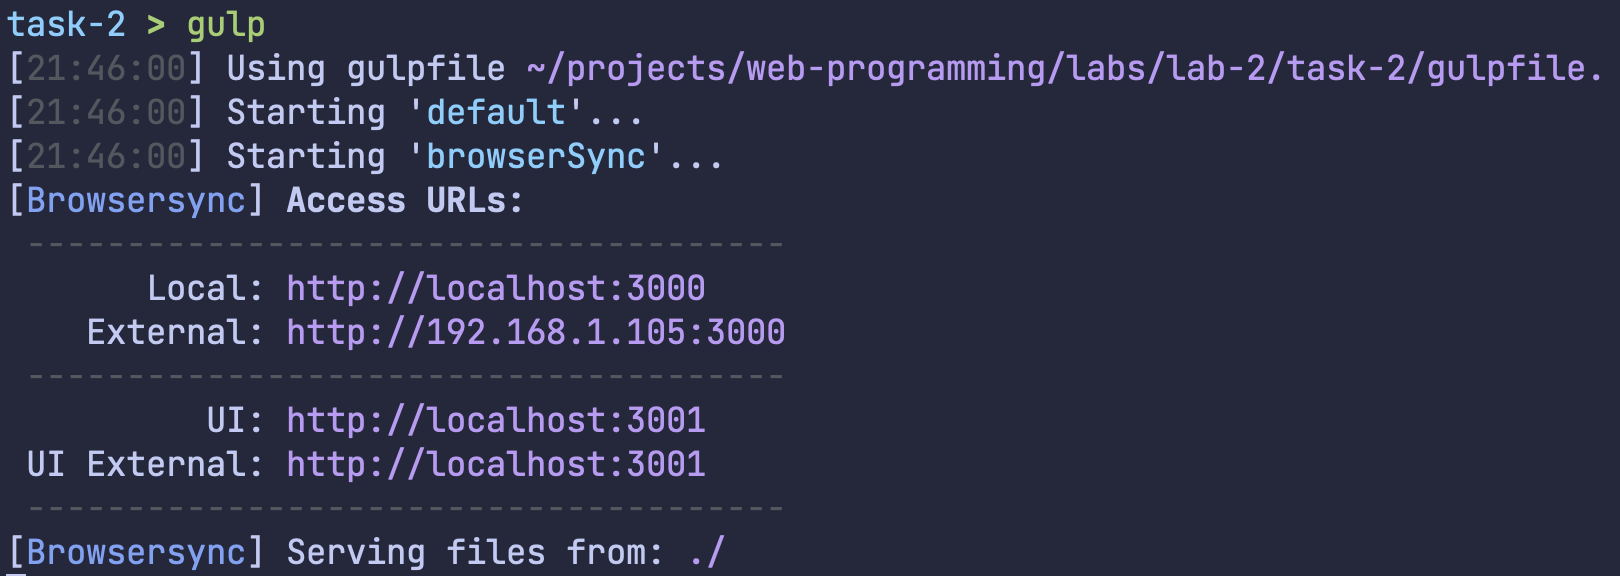
\includegraphics[width=\textwidth]{images/browser-sync.png}
  \caption{Вывод Gulp после запуска}
  \label{fig:browser-sync}
\end{figure}

\begin{figure}[H]
  \centering
  \fbox{
\includegraphics[width=0.9\textwidth]{images/browser-before.png}}
  \caption{Страница браузера до изменения}
  \label{fig:browser-before}
\end{figure}

При изменении содержимого \texttt{index.html} браузер автоматически
перезагрузится с новым содержимым (рис. \ref{fig:browser-after}).

\begin{figure}[H]
  \centering
  \fbox{
\includegraphics[width=0.9\textwidth]{images/browser-after.png}}
  \caption{Страница браузера после изменения}
  \label{fig:browser-after}
\end{figure}

\subsection*{Задание №3}

В данном задании необходимо написать программу клиент, которая показывает
web-страницы одна за другой из списка, при этом в программе можно задавать
адреса страниц и интервал показа.

Для решения данного задания был выбран следующий стек технологий. В качестве
языка программирования был выбран язык C++, поскольку это компилируемый,
статически типизированный язык программирования общего назначения. Он отличается
высокой производительностью, а также переносимостью между системами и
платформами. В добавок ко всему, для этого языка существует множество различных
библиотек, что позволяет использовать C++ в самых различных сферах деятельности.

В качестве библиотеки, с помощью которой будет создаваться графический
пользовательский интерфейс, был выбран фреймворк Qt. Данный фреймворк является
очень популярным решением для разработки графических пользовательских
интерфейсов среди языков C++ и Python. Для него существует множество материалов,
с помощью которых можно найти ответ практически на любой вопрос. Также этот
фреймворк поддерживает все основные операционные системы, что позволяет
запускать приложения, основанные на этом фреймворке, почти повсюду.

На рис. \ref{fig:main-window} изображено главное окно программы. На нем
отображаются все ссылки, добавленные пользователем. Также имеется возможность
создания, редактирования и удаления уже существующих ссылок.

\begin{figure}[H]
  \centering
  \fbox{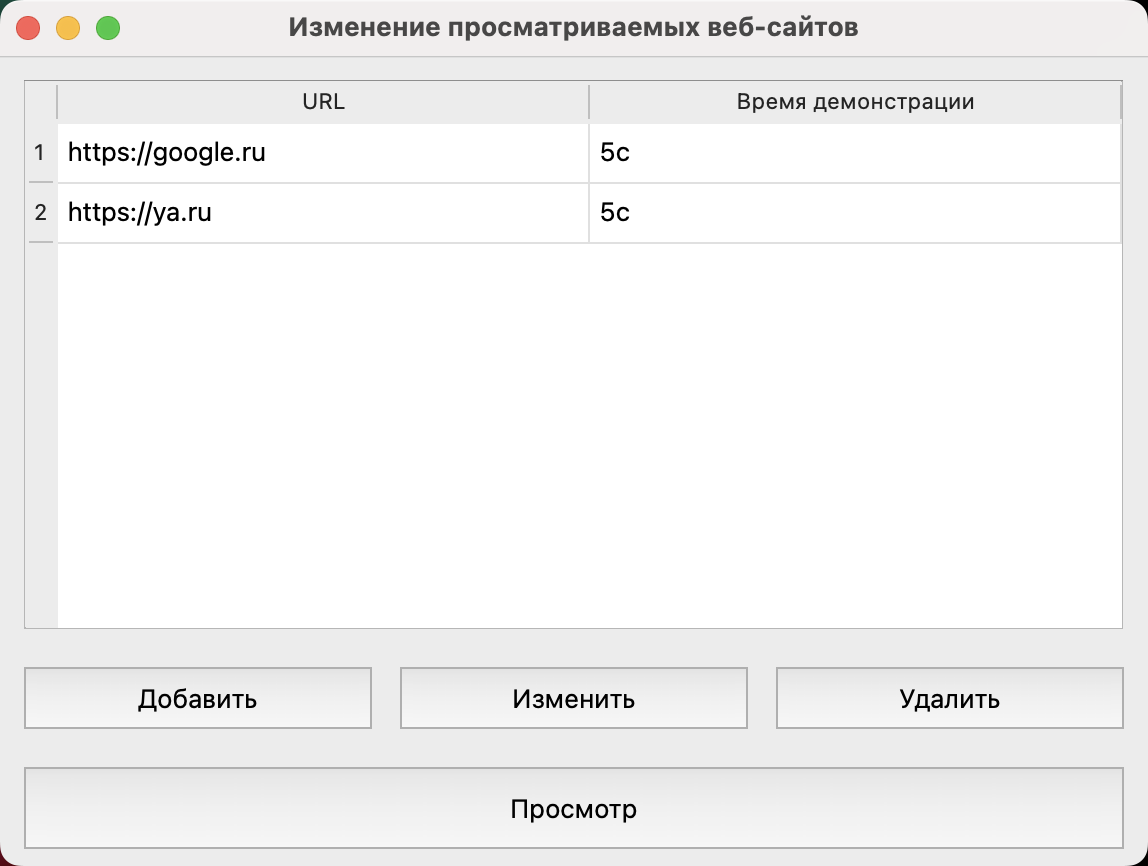
\includegraphics[width=0.8\textwidth]{images/main-window.png}}
  \caption{Главное окно программы}
  \label{fig:main-window}
\end{figure}

При нажатии на кнопку <<Добавить>> пользователю открывается окно, показанное на
рис. \ref{fig:create-window}. В данном окне пользователь должен указать ссылку,
которая будет показана, а также время демонстрации сайта по этой ссылке. Ссылка
должна быть корректной, иначе кнопка <<Сохранить>> не станет активной.

\begin{figure}[H]
  \centering
  \fbox{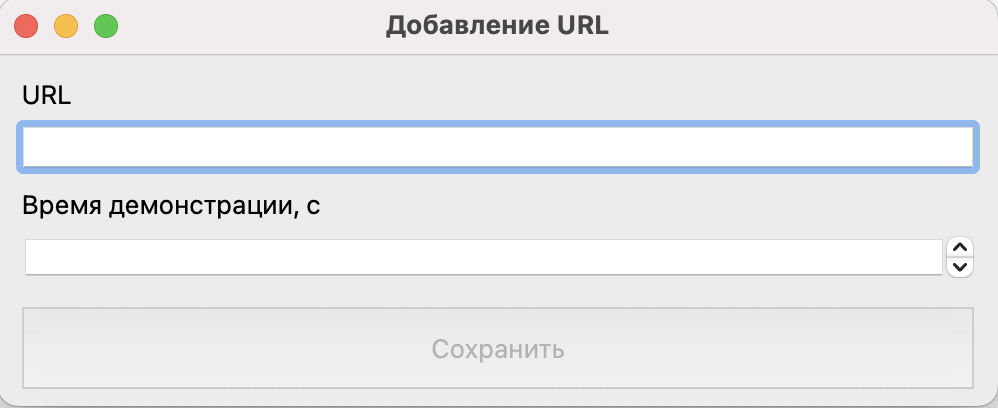
\includegraphics[width=0.7\textwidth]{images/create-window.png}}
  \caption{Окно добавления новой ссылки}
  \label{fig:create-window}
\end{figure}

При двойном нажатии на ссылку или при нажатии на кнопку <<Изменить>>,
открывается окно, изображенное на рис. \ref{fig:change-window}. В данном окне
пользователь может изменить ссылку, которая будет показана, а также время
демонстрации сайта по этой ссылке.

\begin{figure}[H]
  \centering
  \fbox{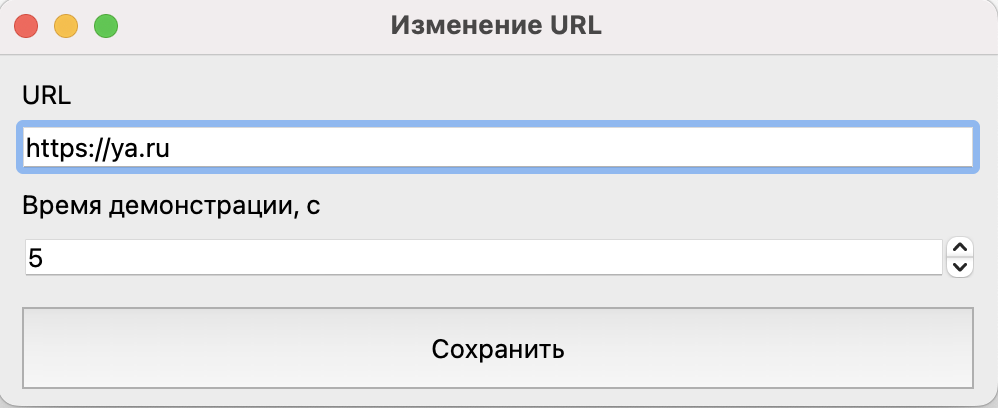
\includegraphics[width=0.7\textwidth]{images/change-window.png}}
  \caption{Окно изменения существующей ссылки}
  \label{fig:change-window}
\end{figure}

При нажатии кнопки <<Удалить>> выбранная ссылка удаляется без какого-либо
дополнительного окна. При нажатии кнопки <<Просмотр>> открывается окно
демонстрации веб-сайтов, изображенное на рис. \ref{fig:viewer-window}. В нем
показывается ссылка, оставшееся время демонстрации, а также сама демонстрируемая
страница. После того, как время выйдет, будет показана следующая ссылка. Если
ссылка была последней, окно демонстрации будет закрыто.

Исходный код приложения, а также скриптов сборки, находится в приложениях
\ref{app:CMakeLists.txt}-\ref{app:website_display_info.hpp}, а также доступен в
\href{https://github.com/danilshvalov/itmo-web-programming}{репозитории на
  GitHub}.

\begin{figure}[H]
  \centering
  \fbox{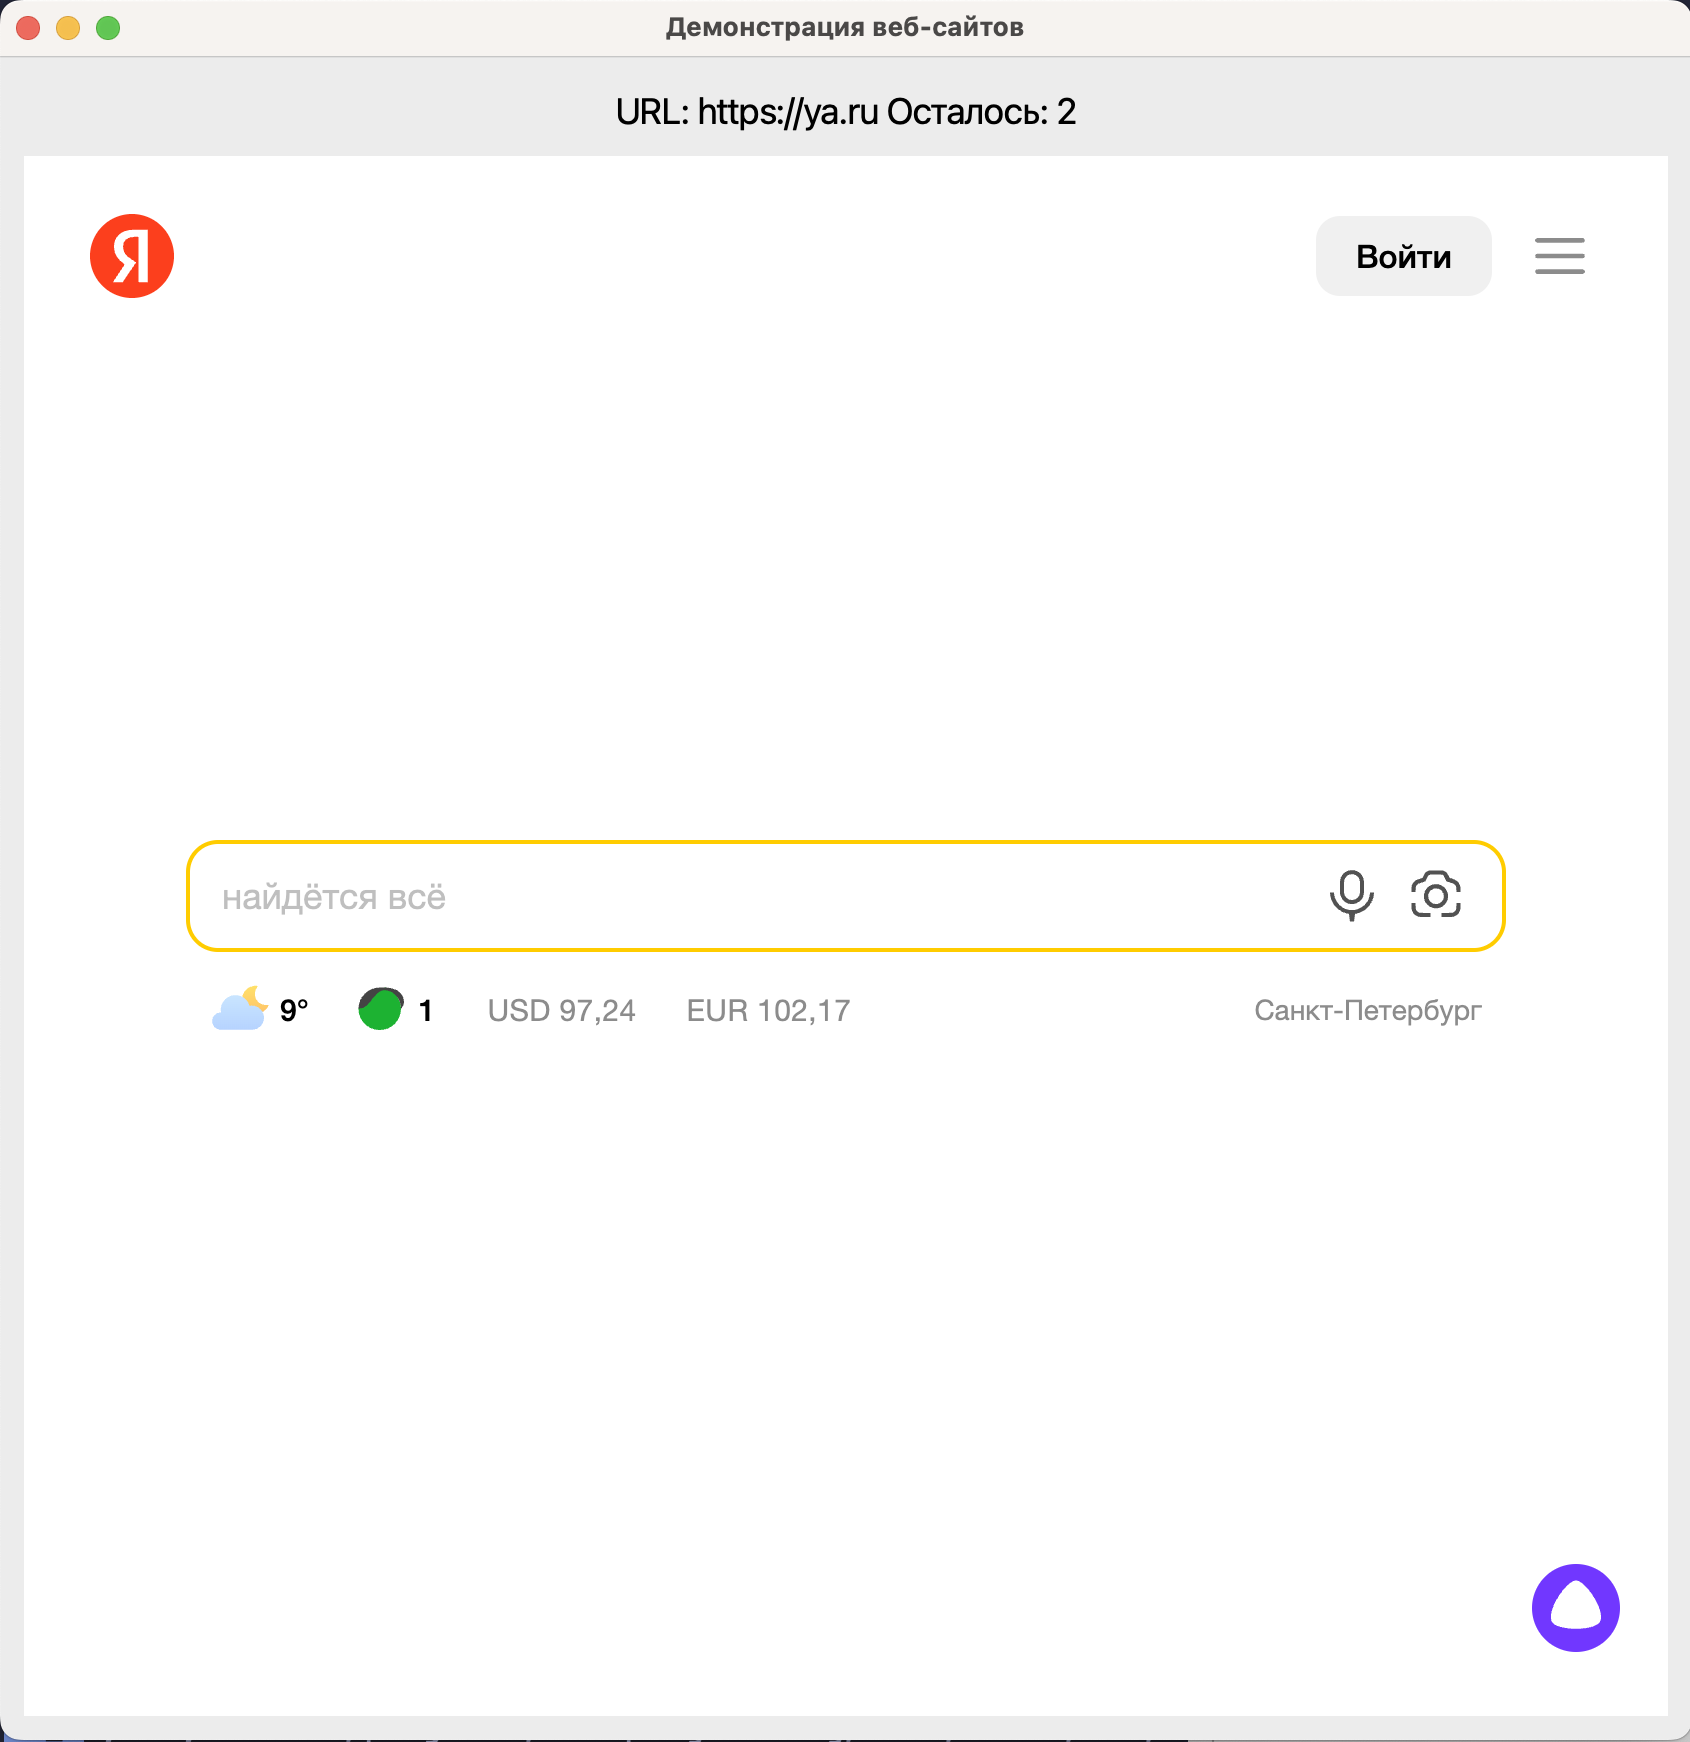
\includegraphics[width=\textwidth]{images/viewer-window.png}}
  \caption{Окно демонстрации веб-сайтов}
  \label{fig:viewer-window}
\end{figure}

\section{Заключение}

\textbf{Вывод}: в данной лабораторной работе я научился использовать систему
контроля версий Git для отслеживания и ведения истории изменения файлов в
проектах, познакомился с инструментом для автоматизации, организации и обработке
задач Gulp, разработал собственное приложение просмотра веб-страниц.

\newpage

\appendix

\titleformat{\section}[display]
{\normalfont\bfseries}
{\centering Приложение\ \thesection}
{0pt}{\centering}
\renewcommand{\thesection}{\Asbuk{section}}

\section{Исходный код package.json}
\label{app:package.json}

\begin{code}
  \inputminted{js}{../task-2/package.json}
\end{code}

\newpage

\section{Исходный код gulpfile.js}
\label{app:gulpfile.js}

\begin{code}
  \inputminted{js}{../task-2/gulpfile.js}
\end{code}

\newpage

\section{Исходный код index.html}
\label{app:index.html}

\begin{code}
  \inputminted{js}{../task-2/index.html}
\end{code}

\newpage

\section{Исходный код CMakeLists.txt}
\label{app:CMakeLists.txt}

\begin{code}
  \inputminted{cmake}{../task-3/CMakeLists.txt}
\end{code}

\newpage

\section{Исходный код main.cpp}
\label{app:main.cpp}

\begin{code}
  \inputminted{cpp}{../task-3/src/main.cpp}
\end{code}

\newpage

\section{Исходный код website\_form.hpp}
\label{app:website_form.hpp}

\begin{code}
  \inputminted{cpp}{../task-3/src/website_form.hpp}
\end{code}

\newpage

\section{Исходный код website\_form.cpp}
\label{app:website_form.cpp}

\begin{code}
  \inputminted{cpp}{../task-3/src/website_form.cpp}
\end{code}

\newpage

\section{Исходный код url\_validator.hpp}
\label{app:url_validator.hpp}

\begin{code}
  \inputminted{cpp}{../task-3/src/url_validator.hpp}
\end{code}

\newpage

\section{Исходный код url\_validator.cpp}
\label{app:url_validator.cpp}

\begin{code}
  \inputminted{cpp}{../task-3/src/url_validator.cpp}
\end{code}

\newpage

\section{Исходный код website\_list\_model.hpp}
\label{app:website_list_model.hpp}

\begin{code}
  \inputminted{cpp}{../task-3/src/website_list_model.hpp}
\end{code}

\newpage

\section{Исходный код website\_list\_model.cpp}
\label{app:website_list_model.cpp}

\begin{code}
  \inputminted{cpp}{../task-3/src/website_list_model.cpp}
\end{code}

\newpage

\section{Исходный код website\_list\_window.hpp}
\label{app:website_list_window.hpp}

\begin{code}
  \inputminted{cpp}{../task-3/src/website_list_window.hpp}
\end{code}

\newpage

\section{Исходный код website\_list\_window.cpp}
\label{app:website_list_window.cpp}

\begin{code}
  \inputminted{cpp}{../task-3/src/website_list_window.cpp}
\end{code}

\newpage

\section{Исходный код website\_viewer.hpp}
\label{app:website_viewer.hpp}

\begin{code}
  \inputminted{cpp}{../task-3/src/website_viewer.hpp}
\end{code}

\newpage

\section{Исходный код website\_viewer.cpp}
\label{app:website_viewer.cpp}

\begin{code}
  \inputminted{cpp}{../task-3/src/website_viewer.cpp}
\end{code}

\newpage

\section{Исходный код table\_list\_model.hpp}
\label{app:table_list_model.hpp}

\begin{code}
  \inputminted{cpp}{../task-3/src/table_list_model.hpp}
\end{code}

\newpage

\section{Исходный код website\_display\_info.hpp}
\label{app:website_display_info.hpp}

\begin{code}
  \inputminted{cpp}{../task-3/src/website_display_info.hpp}
\end{code}

\end{document}
